
\documentclass{article}
\usepackage[T1]{fontenc}
\usepackage[utf8]{inputenc}
\usepackage[spanish]{babel}
\usepackage{amssymb, amsmath, amsbsy}
\usepackage{graphicx}
\title{Ligra\\Algoritmos paralelos}
\author{Peto Gutierrez Emmanuel}
\begin{document}
\maketitle

\section{Tiempo}

\begin{table}[htbp]
\begin{center}
\begin{tabular}{|l|l|}
\hline
Marca & Huawei \\ \hline
Sistema operativo & Ubuntu 20.04 \\ \hline
Procesador & AMD Ryzen 7, 4800 \\ \hline
Número de procesadores & 16 \\ \hline
Número de núcleos & 8 \\ \hline
RAM & 16 GB \\ \hline

\end{tabular}
\caption{Características del equipo.} \label{table:1}
\end{center}
\end{table}

\subsection{Un millón de vértices}

Al crear ejemplares se utilizó el ejecutable \texttt{./randLocalGraph -m <m> <n> <archivo>}. El ejemplar generado para las pruebas tiene $10^6$ vértices y $2 \times 10 ^7$ aristas.

\begin{table}[htbp]
\begin{center}
\begin{tabular}{|l|l|l|l|l|l|}
\hline
\textbf{Prueba} & \textbf{1} & \textbf{2} & \textbf{3} & \textbf{4} & \textbf{5} \\ \hline
\textbf{Tiempo 1 (s)} & 0.0181 & 0.018 & 0.0179 & 0.018 & 0.0181 \\ \hline
\textbf{Tiempo 2 (s)} & 0.0194 & 0.0208 & 0.0192 & 0.0205 & 0.02 \\ \hline
\textbf{Tiempo 3 (s)} & 0.0198 & 0.0202 & 0.0218 & 0.02 & 0.0196 \\ \hline

% 0.0181	0.018	0.0179	0.018	0.0181	0.0194	0.0208	0.0192	0.0205	0.02	0.0198	0.0202	0.0218	0.02	0.0196

\end{tabular}
\caption{Tiempos de ejecución para ejemplar de tamaño $10^6$, sin compartir recursos.} \label{table:2}
\end{center}
\end{table}

Los tiempos de ejecución en segundos para el ejemplar de orden $10^6$ se muestran en el Cuadro \ref{table:2}. La gráfica con los resultados se muestra en la Figura \ref{fig:grafico}, donde los puntos del 1 al 5 son de la primera fila, los de la 6 a la 10 son de la segunda fila y del 11 al 15 son de la tercera fila. El promedio de los datos es 0.0194 s.

Al momento de ejecutar BFS sólo se tenía abierto \texttt{Gedit} y \texttt{Archivos}.

\begin{figure}[htbp]

\center

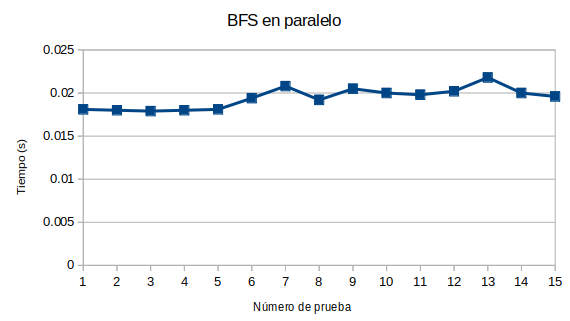
\includegraphics[scale=0.5]{imagenes/grafico1M}

\caption{Gráfica de puntos y líneas de los tiempos de ejecución para BFS en paralelo.} \label{fig:grafico}

\end{figure}

Ahora se ejecutará BFS pero teniendo en ejecución otros programas y se calculará el tiempo.

\begin{table}[htb]
\begin{center}
\begin{tabular}{|l|l|l|l|l|l|}
\hline
\textbf{Prueba} & \textbf{1} & \textbf{2} & \textbf{3} & \textbf{4} & \textbf{5} \\ \hline
\textbf{Tiempo 1 (s)} & 0.0201 & 0.0185 & 0.019 & 0.0202 & 0.0203 \\ \hline
\textbf{Tiempo 2 (s)} & 0.0212 & 0.0229 & 0.0223 & 0.0225 & 0.0213 \\ \hline
\textbf{Tiempo 3 (s)} & 0.0231 & 0.0336 & 0.0224 & 0.0228 & 0.0219 \\ \hline

% 0.0201	0.0185	0.019	0.0202	0.0203	0.0212	0.0229	0.0223	0.0225	0.0213	0.0231	0.0336	0.0224	0.0228	0.0219

\end{tabular}
\caption{Tiempos de ejecución para ejemplar de orden $10^6$, compartiendo recursos con otros programas.} \label{table:3}
\end{center}
\end{table}

En el Cuadro \ref{table:3} se encuentran los resultados de ejecutar BFS con un ejemplar de orden $10^6$ compartiendo recursos con otros programas. Al momento de ejecutar BFS se tenían abiertos los siguientes programas:

\begin{itemize}
\item Visual Studio Code.
\item Chrome con una pestaña en un video de Youtube en reproducción y otra pestaña con Facebook.
\item Spotify reproduciendo una canción.
\item Editor de textos.
\item Visor de documentos.
\end{itemize}

En este caso el promedio del tiempo de ejecución es 0.0221 s, lo cual es ligeramente mayor a 0.0194 s, que es el tiempo promedio sin tener otros programas en ejecución. En la Figura \ref{fig:grafico2} se grafican los resultados del Cuadro \ref{table:3} de color naranja y los del Cuadro \ref{table:2} de color azul. Nótese que la línea naranja queda por encima de la línea azul.

\begin{figure}[htbp]

\center

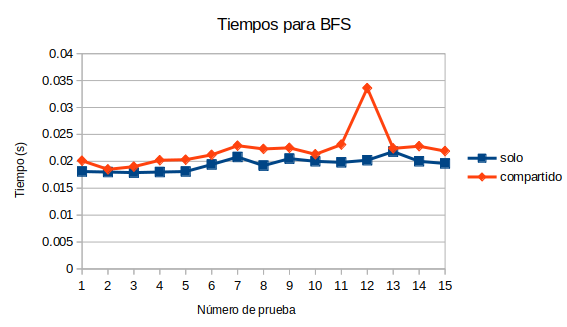
\includegraphics[scale=0.5]{imagenes/grafico2}

\caption{La línea azul representa los tiempos cuando no se usan otros programas, mientras que la línea naranja representa los tiempos cuando se ejecutan otros programas en la computadora.} \label{fig:grafico2}

\end{figure}

\subsection{Resultados de Juan García}

Ahora, se compararán los datos del compañero Juan Garcia con los míos. Las características de su equipo se encuentran en el Cuadro \ref{table:juanpc}. Los resultados de sus pruebas se encuentran en el Cuadro \ref{table:juanres}, las cuales se realizaron con la gráfica de orden $10^6$ sin compartir recursos con otros programas.

\begin{table}[htbp]
\centering
\begin{tabular}{|l|c|}
\hline
Generación del procesador & AMD A6-9225 (7ma generación) \\ \hline
Número de procesadores & 2 \\ \hline
Número de nucleo & 2 \\ \hline
RAM & 8gb \\ \hline
\end{tabular} \quad
\caption{Detalles y especificaciones del hardware con el que cuenta la computadora en donde se realizaron las pruebas.} \label{table:juanpc}
\end{table}

\begin{table}[htbp]
\begin{tabular}{|c|c|c|c|c|}
\hline
\textbf{Prueba 1} & \textbf{Prueba 2} & \textbf{Prueba 3} & \textbf{Prueba 4} & \textbf{Prueba 5} \\ \hline
0.0845 & 0.0849 & 0.0859 & 0.0859 & 0.0854 \\ \hline
0.0941 & 0.0963 & 0.0969 & 0.0962 & 0.0946 \\ \hline
0.0935 & 0.0917 & 0.0923 & 0.0928 & 0.0927 \\ \hline
\end{tabular}
% 0.0845	0.0849	0.0859	0.0859	0.0854	0.0941	0.0963	0.0969	0.0962	0.0946	0.0935	0.0917	0.0923	0.0928	0.0927
\caption{Pruebas sin compartir recursos} \label{table:juanres}
\end{table}

En el equipo de Juan el tiempo promedio es de 0.0911 s, que es mayor al tiempo promedio obtenido en mi equipo (0.0194 s). Esto tiene sentido porque su equipo tiene 2 procesadores y 2 núcleos y el mío 16 procesadores y 8 núcleos.

En la Figura \ref{fig:compa} se muestran los tiempos obtenidos en ambos equipos en una gráfica de puntos y líneas.

\begin{figure}[htbp]

\center

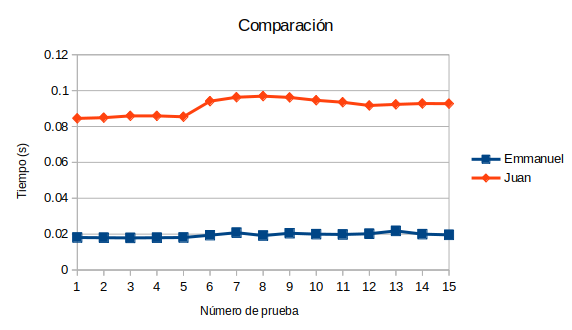
\includegraphics[scale=0.5]{imagenes/comparacion}

\caption{Resultados en diferentes equipos.} \label{fig:compa}

\end{figure}

\subsection{Ejemplar de tamaño máximo}

También se creó un ejemplar con 6.2$\times 10^7$ vértices y 6.2$\times 10^8$ aristas; después se intentó crear un ejemplar con 6.3$\times 10^7$ vértices y 6.3$\times 10^8$ aristas, pero la ejecución del programa dio como resultado: \texttt{Terminado (killed)}, o sea, se mató el proceso antes de que terminara (ver Figura \ref{fig:killed}). Esto implica que el máximo número de vértices que puede crear mi computadora está entre 6.2$\times 10^7$ y 6.3$\times 10^7$ (entre 62 y 63 millones).

\begin{figure}[htbp]

\center

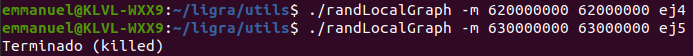
\includegraphics[width=\linewidth]{imagenes/limite2}

\caption{Proceso terminado.} \label{fig:killed}

\end{figure}

Aunque el ejemplar más grande que se pudo construir tiene 6.2$\times 10^7$ vértices, se utilizó uno de 3.5$\times 10^7$. Esto es porque al ejecutar BFS en el ejemplar más grande, el sistema operativo ``mata'' al proceso (muestra: \texttt{Terminado (killed)}). Los resultados de la ejecución se muestran en el Cuadro \ref{table:4}. El promedio de los tiempos es 1.239 s.

\begin{table}[htbp]
\begin{center}
\begin{tabular}{|l|l|l|l|l|l|}
\hline
\textbf{Prueba} & \textbf{1} & \textbf{2} & \textbf{3} & \textbf{4} & \textbf{5} \\ \hline
\textbf{Tiempo 1 (s)} & 1.25 & 1.24 & 1.23 & 1.24 & 1.23 \\ \hline
\textbf{Tiempo 2 (s)} & 1.24 & 1.24 & 1.24 & 1.24 & 1.26 \\ \hline
\textbf{Tiempo 3 (s)} & 1.23 & 1.23 & 1.24 & 1.23 & 1.25 \\ \hline

% 1.25	1.24	1.23	1.24	1.23	1.24	1.24	1.24	1.24	1.26	1.23	1.23	1.24	1.23	1.25

\end{tabular}
\caption{Tiempos de ejecución para ejemplar de orden 3.5$\times 10^7$, sin compartir recursos.} \label{table:4}
\end{center}
\end{table}

Ahora, se ejecutará BFS en el mismo ejemplar pero ejecutando otros programas en la computadora, igual que con el de un millón de vértices: Visual Studio Code, Chrome, etc. Los resultados se muestran en el Cuadro \ref{table:5}. El promedio de los tiempos es 1.361 s, que es mayor al promedio cuando no se ejecuta ningún otro programa (1.239 s).

\begin{table}[htbp]
\begin{center}
\begin{tabular}{|l|l|l|l|l|l|}
\hline
\textbf{Prueba} & \textbf{1} & \textbf{2} & \textbf{3} & \textbf{4} & \textbf{5} \\ \hline
\textbf{Tiempo 1 (s)} & 1.39 & 1.37 & 1.36 & 1.38 & 1.37 \\ \hline
\textbf{Tiempo 2 (s)} & 1.36 & 1.35 & 1.33 & 1.35 & 1.33 \\ \hline
\textbf{Tiempo 3 (s)} & 1.35 & 1.38 & 1.37 & 1.35 & 1.38 \\ \hline

%1.39	1.37	1.36	1.38	1.37	1.36	1.35	1.33	1.35	1.33	1.35	1.38	1.37	1.35	1.38

\end{tabular}
\caption{Tiempos de ejecución para ejemplar de orden 3.5$\times 10^7$, compartiendo recursos.} \label{table:5}
\end{center}
\end{table}

La Figura \ref{fig:grafico3} muestra las gráficas de puntos y líneas de los tiempos obtenidos. La línea azul es cuando se ejecuta BFS solo y la naranja es cuando se comparten recursos con otros programas.

\begin{figure}[htbp]

\center

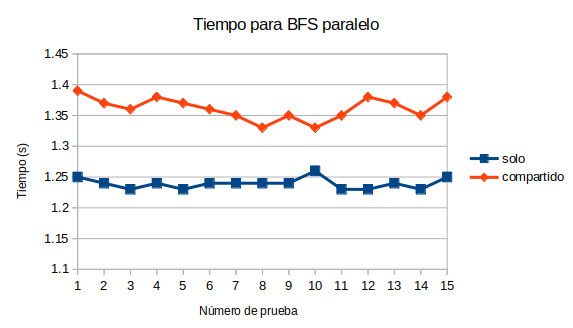
\includegraphics[scale=0.5]{imagenes/grafico3}

\caption{La línea azul representa los tiempos cuando no se usan otros programas, mientras que la línea naranja representa los tiempos cuando se ejecutan otros programas.} \label{fig:grafico3}

\end{figure}

\section{Temperatura}

En esta sección se leerá la temperatura de los procesadores cuando se ejecutan diferentes procesos.

\textbf{1.} Primero se obtiene la temperatura cuando no se está ejecutando ningún programa y sólo se están ejecutando los procesos del sistema operativo, ver Figura \ref{fig:so}.

\begin{figure}[htbp]

\center

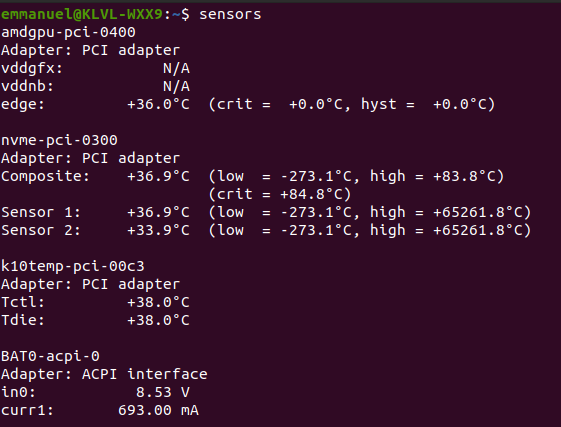
\includegraphics[scale=0.5]{imagenes/temp1}

\caption{Temperatura cuando no se ejecuta ningún programa.} \label{fig:so}

\end{figure}

\textbf{2.} Se abrió \textit{Android Studio} y se ejecutó el emulador del celular, como se observa en la Figura \ref{fig:android}. Primero se registró la temperatura sin un sistema de ventilación externa y se muestra en la Figura \ref{fig:temp2}.

\begin{figure}[htbp]

\center

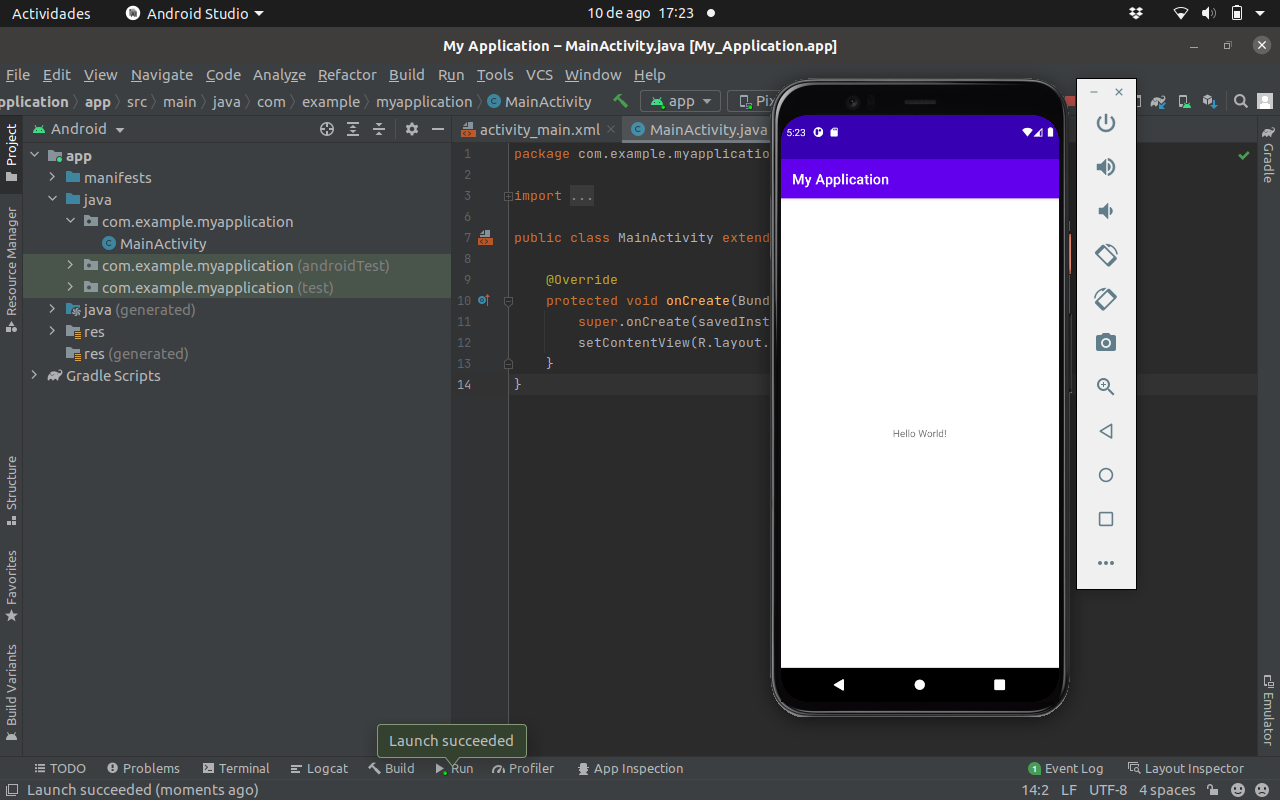
\includegraphics[width=\linewidth]{imagenes/android}

\caption{Android Studio junto con emulador de celular.} \label{fig:android}

\end{figure}

\begin{figure}[htbp]

\center

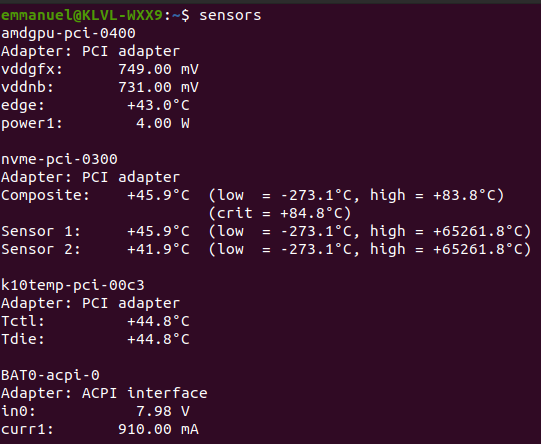
\includegraphics[scale=0.5]{imagenes/temp2}

\caption{Temperatura cuando se ejecuta Android Studio y el emulador, sin sistema de ventilación externa.} \label{fig:temp2}

\end{figure}

\textbf{3.} Luego, teniendo \textit{Android Studio} y el emulador como en el caso \textbf{2.}, se conectó un enfriador para laptop y un ventilador, como se muestra en la Figura \ref{fig:ventiladores}. Las temperaturas registradas en este caso se muestran en la Figura \ref{fig:temp3} y se puede observar que son menores que cuando no se usa la ventilación. Por ejemplo, en \texttt{k10temp-pci-00c3} la diferencia de temperatura es de dos grados.

A partir de este punto se dejó de usar la ventilación externa.

\begin{figure}[htbp]

\center

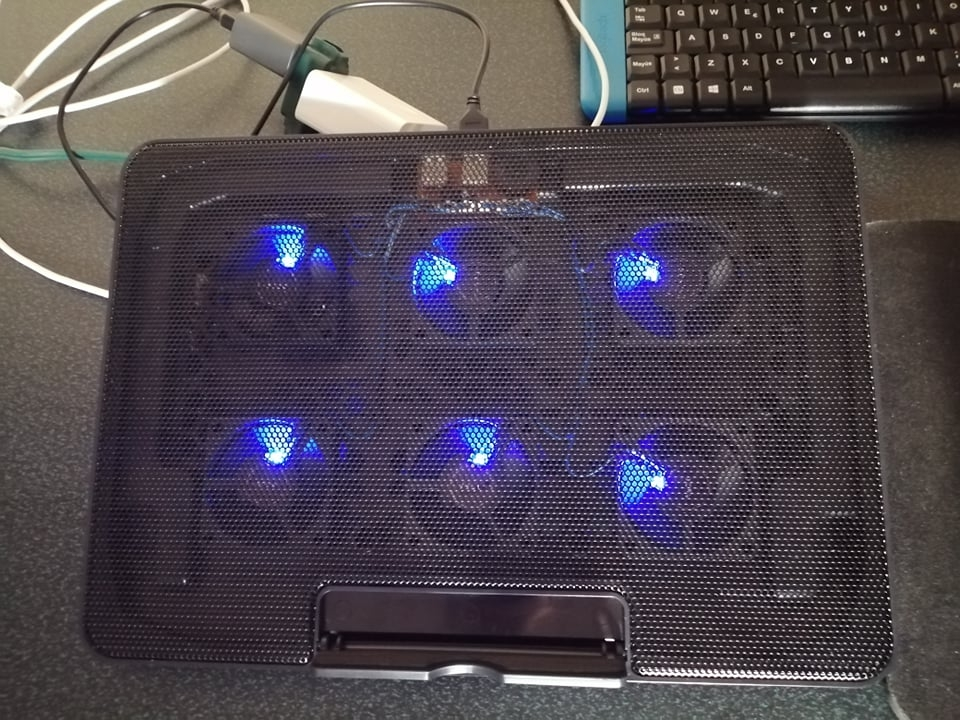
\includegraphics[width=0.45\linewidth]{imagenes/placa}
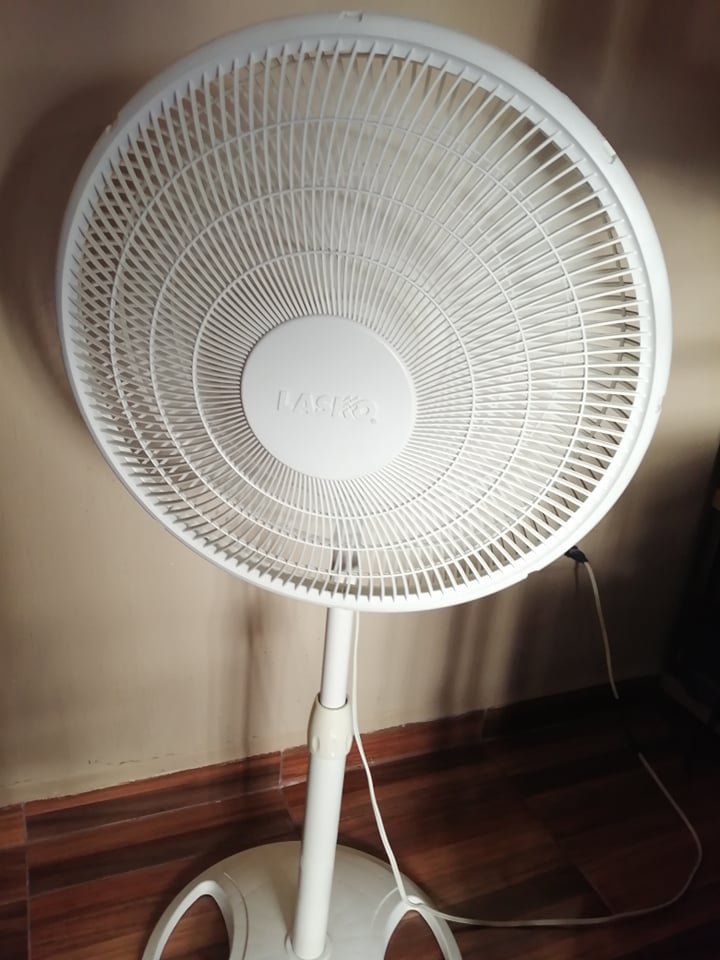
\includegraphics[width=0.45\linewidth]{imagenes/ventilador}

\caption{Base enfriadora para laptop y ventilador.} \label{fig:ventiladores}

\end{figure}

\begin{figure}[htbp]

\center

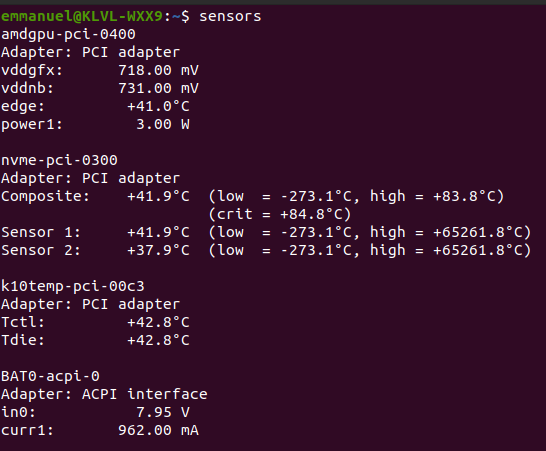
\includegraphics[scale=0.5]{imagenes/temp3}

\caption{Temperatura con Android Studio y emulador, usando ventilación.} \label{fig:temp3}

\end{figure}

Se registraron las temperaturas de los procesadores al ejecutar BFS de Ligra usando el ejemplar de 35 millones de vértices y 350 millones de aristas. En la Figura \ref{fig:temp4} se observan las temperaturas antes de ejecutar el algoritmo (izquierda), mientras se ejecutaba (centro) y al final de su ejecución (derecha), aproximadamente a 10 segundos de haber terminado.

El mayor cambio se da en \texttt{k10temp-pci-00c3}, donde inicia en 40º C, de ahí sube a 43.9º C mientras se está ejecutando y termina en 56.1º C.

\begin{figure}[htbp]

\center

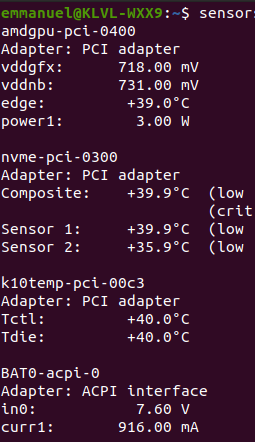
\includegraphics[width=0.3\linewidth]{imagenes/temp4_1}
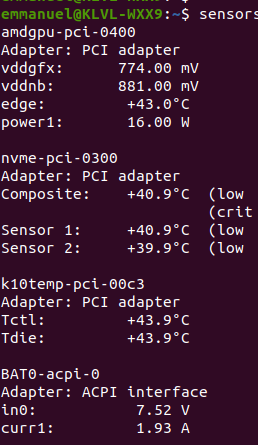
\includegraphics[width=0.3\linewidth]{imagenes/temp4_2}
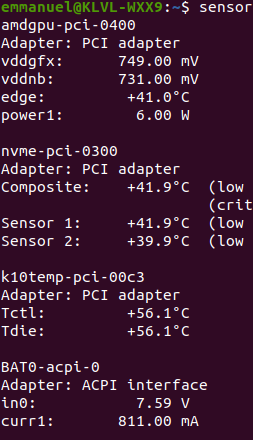
\includegraphics[width=0.3\linewidth]{imagenes/temp4_3}

\caption{Temperaturas al ejecutar BFS de Ligra.} \label{fig:temp4}

\end{figure}

Finalmente, se tomó la temperatura al ejecutar el programa \texttt{cod01.c} de la Práctica 1. El programa lanza 100 hilos y cada uno ejecuta un \texttt{printf} dentro de un loop infinito (\texttt{while(1)}). El resultado se observa en la Figura \ref{fig:temp5}, donde la temperatura de \texttt{k10temp-pci-00c3} es de 63.1º C.

\begin{figure}[htbp]

\center

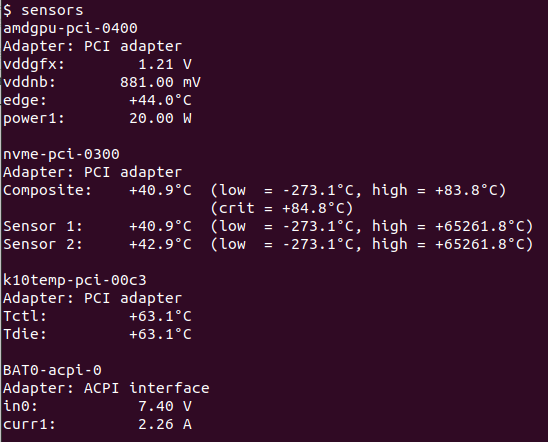
\includegraphics[scale=0.5]{imagenes/temp5}

\caption{Temperaturas al ejecutar 100 hilos con un loop infinito.} \label{fig:temp5}

\end{figure}

\end{document}

